\section{Random Walk on a Grid} 
A `particle' takes a random walk on a $4 \times 8$ grid. At each step of the walk, the particle may move up, down, left, or right with equal probability. The particle continues this process until it exits the grid. If the particle exits the top of the grid, the particle scores 1 point for the walk. If the particle exits the left, bottom or right sides of the grid, the particle scores 0 points for the walk. 


\begin{center}
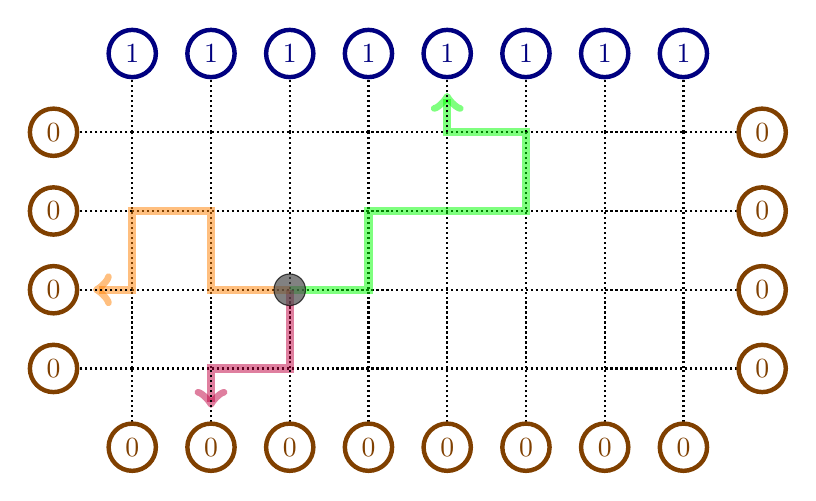
\begin{tikzpicture}
    \pgfmathsetmacro{\N}{8}
    \pgfmathsetmacro{\M}{4}
    \draw[thick, densely dotted] (1,1) grid (\N,\M);
    \draw[line width = 3,color = green, opacity = .5,->] (3,2) -- (4,2) --(4,3) --(5,3) -- (6,3) --(6,4) --(5,4) -- (5,4.5);
    \draw[line width = 3,color = purple, opacity = .5,->] (3,2) -- (3,1) --(2,1) --(2,0.5);
    \draw[line width = 3,color = orange, opacity = .5,->] (3,2) -- (2,2) --(2,3) --(1,3) -- (1,2)--(0.5,2);
    % Right
    \foreach \j in {1,...,\M}
    {
    \draw[thick, densely dotted] (\N+1,\j) -- (\N,\j);
    \draw[ultra thick,color=orange!50!black,fill = white] (\N+1,\j) node {0} circle (.3);
    }
    % Top
    \foreach \i in {1,...,\N}
    {
        \draw[thick, densely dotted] (\i,\M) -- (\i,\M+1);
        \draw[ultra thick,color=blue!50!black,fill = white] (\i,\M+1) node {1} circle (.3);
    }
    % Left
    \foreach \j in {1,...,\M}
    {
        \draw[thick, densely dotted] (1,\j) -- (0,\j);
        \draw[ultra thick,color=orange!50!black,fill = white] (0,\j) node {0} circle (.3);
    }
    % Bottom
    \foreach \i in {1,...,\N}
    {
        \draw[thick, densely dotted] (\i,0) -- (\i,1);
        \draw[ultra thick,color=orange!50!black,fill = white] (\i,0) node {0} circle (.3);
    }
    \draw[color = black,fill=black!70!white,opacity = .7] (3,2) circle  (.2);
\end{tikzpicture}
\end{center}
The figure shows three sample paths of the random walk that all begin at the initial point (3,2). For the red path, the particle (randomly) takes the steps $(\downarrow, \leftarrow, \downarrow)$, and exits the grid at the bottom scoring zero points for the walk. The other paths are the results of the steps listed below
\begin{align*}
&\text{Steps: }  (\downarrow \ \leftarrow \ \downarrow) &&\text{(See red path)} && \text{Exit: Bottom} && \text{Score: 0}\\
&\text{Steps: }  (\leftarrow \ \uparrow \ \leftarrow \ \downarrow \ \leftarrow) &&\text{(See orange path)} && \text{Exit: Left} && \text{Score: 0}\\
&\text{Steps: }  (\rightarrow \ \uparrow \ \rightarrow \ \rightarrow \ \uparrow \ \leftarrow \ \uparrow) &&\text{(See green path)}&& \text{Exit: Top} && \text{Score: 1}
\end{align*}

\noindent Compute the expected score of the particle as a function of the starting coordinates.\\

\noindent \textit{Hint:} For each starting point, you may estimate the expected score of the particle by simulating many, many random paths and taking their average score.\\

\noindent\textit{Bonus:} In this project, we have computed the solution to a problem by simulating many random events. This `indirect' approach is always computationally inefficient, so it is often worth looking for a `direct' approach. For this problem, there \textit{is} a method of computing the solution directly. Can you find it?

